\documentclass[../main.tex]{subfiles}
\begin{document}
\section{\label{sect:RQFT}Applications in relativistic physics: non-equilibrium QFT and finite density QCD}


After interest in applying CL to relativistic physics expanded with a series of papers on finite
density QCD in the mid-2000s (see Refs.~\cite{PhysRevLett95202003,PhysRevD75045007,JHEP200809018,%
AartsPRL102131601,JHEP200905052,Lattice2012Aarts}),
much work has gone into the testing of the methodology, its capabilities, and its limitations. While CL has
successfully circumvented the sign problem in a few key areas, it suffers from some of the problems discussed
previously in \secref{formalism}. As a result, recent emphasis has been on determining regions of
applicability and adjusting the method in order to prevent ``excursions" of the Langevin evolution into the
complex plane and ensure convergence to the correct solution.

While the aim of this review is to focus on applications of CL to nonrelativistic quantum many-body problems,
in this section we provide a very brief summary of selected applications to relativistic field theories.
For more on the use of CL in relativistic physics, we refer the reader to Refs.~\cite{Seiler2017StatusOfCL,Lattice2012Aarts}.

%%%%%%%%%%%%%%%%%%%%%%%%%%%%%
\subsection{QCD-inspired toy models}
In Lattice QCD, the main promise of CL is its potential to explore regions of the QCD phase diagram which are currently inaccessible due to a sign
problem. Historically, the emphasis has been on the region of non-zero quark chemical potential, which suffers from a complex phase problem,
but also to real-time dynamics~\cite{Berges:2006xc,Berges:2007nr,deAguiar:2010ue}
and the coupling to a topological charge (see Ref.~\cite{Seiler2017StatusOfCL}) are also of great interest.
While the CL method has not yet been able to produce detailed solutions in this region (some attempts notwithstanding, see below),
 a number of simpler models have been successfully studied. We mention here just a few of those cases.

\begin{itemize}

\item {\it XY model} --
Results using CL in the three-dimensional XY model at non-zero chemical potential~\cite{JHEP20100820} turn out to be very promising for the ordered phase, but fail to reproduce known answers for the disordered (high-temperature) phase. The XY model is useful for testing CL because the sign problem can be circumvented in other ways, for example using dual variables in a world-line formulation.
Moreover, the model is very sensitive to instabilities in the algorithm - just as heavy-dense QCD is. The instabilities in the algorithm can be eliminated by the addition of adaptive stepsize to the Langevin evolution, which had been shown to work in the three-dimensional XY model at non-zero chemical potential and in the heavy-dense limit of QCD (HQCD)~\cite{AARTS2010154}. Adaptive step size prevents the CL trajectory from changing by too large a value, thereby diverting from the real axis and into the complex plane.
Another way to improve the convergence of CL in the XY model is by dynamic stabilization, which forces the Langevin trajectory to remain near the real axis by means of unitary transformations~\cite{Lattice2017AttanasioJager}. These transformations modify the drift function to prevent large excursions in the imaginary direction~\cite{Seiler2017StatusOfCL,Lattice2016AttanasioJager}.


\item {\it SU(3) spin model} --
The three-dimensional SU(3) spin model is an effective Polyakov loop model for QCD at nonzero temperature and density. It suffers from a sign problem at nonzero chemical potential and typically reweighting or the phase-quenched approximation are used to study its behavior. Complex Langevin was used to successfully address this model, originally in Ref.~\cite{PhysRevLett.55.2242} and more recently in Refs.~\cite{Aarts2012SU3,Aarts:2012ft} with remarkable accuracy across a phase transition, with particular emphasis on the justification of the approach. Results are shown in \figref{su3_plots} along with the average phase factor in the phase-quenched theory, which deteriorates quickly with increasing system size. The success of CL within this model underlines its ability to solve severe sign problems.
%
\begin{figure}
  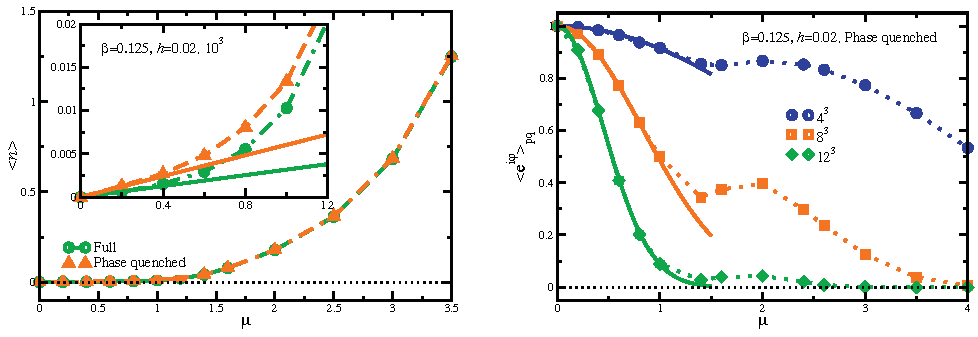
\includegraphics[width=\textwidth]{./4applications-REL/fig11.pdf}
  \caption{(Left) SU(3) spin-model in the full and the phase-quenched theory as a function of $\mu$. The inset shows a close-up of the small $\mu$ region. The lines are the predicted linear dependence for small $\mu$ in excellent agreement with the CL results. (Right) Average phase factor as a function of $\mu$ for the SU(3) model, highlighting the severeness of the sign problem that the CL is able to solve. See Ref.~\cite{Aarts2012SU3}.}
  \label{fig:su3_plots}
\end{figure}


\item {\it Random matrix theory} --
Random matrix theory (RMT) models of finite density QCD are another way to study the accessibility of CL to outstanding problems in QCD. Such models can be constructed with complex fermion determinants and feature finite density phase transitions, where many problems with CL can arise. Some recent work on one of these models suggests that with suitably designed
reweighting methods, CL is able to fully reproduce the known analytical solution to the model at the finite phase transition~\cite{2017EPJWC13707030B}.

\item {\it Polyakov loop model} --
Attempts to control and stabilize the Langevin evolution on these toy models for QCD have led to breakthroughs in methodology. One - already discussed above - is dynamic stabilization, which modifies the drift term of the Langevin equation in order to control fluctuations that might lead the simulation into the complex plane. Another, gauge cooling~\cite{SeilerGaugeCooling, Bongiovanni:2013nxa, Bongiovanni:2014rna}, has allowed for a successful simulation of a QCD-like gauge model, namely the Polyakov loop model, at finite density.


\end{itemize}

%%%%%%%%%%%%%%%%%%%
\subsection{$3+1$ dimensional QCD at finite chemical potential}

One of the early attempts to calculate the properties of full QCD at finite chemical potential is the work of Ref.~\cite{Sexty:2013ica}.
Later on, the results of Ref.~\cite{Lattice2015KogutSinclair} suggested CL with gauge cooling produces trustworthy
solutions for $3+1$ dimensional QCD at zero temperature and finite chemical potential. Work on this same system using a
combination of adaptive stepsize and gauge cooling to prevent runaways in the complex plane for weak coupling showed
promise. In fact, the results share some important physical traits with the system. However, known results were not accurately
recovered. To be more specific, the observation of the transition from hadronic to nuclear matter (at $\mu \approx m_{N}/3$) is visible, as is
evidence of saturation at large chemical potential~\cite{LATTICE2016PROCSinclairKogut}. The zero chemical potential limit
disagreed with known results, but to a very small degree. With larger lattices and lower coupling, the known results are
still not accurately recovered. This has been traced back to the fact that these calculations suffer from
the appearance of zeroes in the fermion determinant in this regime~\cite{Lattice2017KogutSinclair} (see also~\cite{Sinclair:2018rbk, Kogut:2019qmi}).

Another way to treat the singular drift problem is to deform the fermion matrix in order to avoid zeroes in the
determinant and therefore poles in the complex plane that might cause the solution to diverge. This solution can also
be combined with gauge cooling to prevent the excursion problem, and recent work combining these two adaptations to
a CL evolution of $3+1$ dimensional QCD at low temperature and finite density indeed looks
promising~\cite{Nagata:2016alq, 2018EPJWC17507017N}.


%
\begin{figure}[t]
  \centering
  \includegraphics[width=0.49\columnwidth]{./4applications-REL/DensityQCDFiniteMuSexty.pdf}
  \includegraphics[width=0.49\columnwidth]{./4applications-REL/PolyakovQCDFiniteMuSexty.pdf}
  \caption{\label{fig:SextyPlots} Comparison of the average quark densities (left) and the Polyakov loop (right) as obtained from HQCD and a CL
  study of full QCD with staggered fermions, see Ref.~\cite{Sexty:2013ica}.}
\end{figure}

%%%%%%%%%%%%%%%%%%%%
\subsection{Low-dimensional QCD at non-zero chemical potential}

The CL approach has been applied to low-dimensional toy models for the matter sector of QCD~\cite{Pawlowski:2013pje,Pawlowski:2013gag} 
and it has now also been shown to be effective in low-dimensional QCD calculations. To be more specific, 
in $0+1$ dimensional QCD, the quark density and chiral condensate have been computed using CL, with gauge cooling used to prevent the simulation from deviating in the imaginary direction~\cite{Bloch:2015coa}. Simulations in $1+1$ dimensional QCD have also correctly calculated the chiral condensate in the thermodynamic limit~\cite{JHEP0820101017}. In recent years, work on combining reweighting techniques with CL have expanded the range of applications of the method to previously inaccessible parameter space in QCD, allowing for greater ranges of values for the mass, temperature, and chemical potential in $1+1$-dimensional QCD~\cite{Bloch:2017sfg,PhysRevD95054509}. 

%%%%%%%%%%%%%%%%%%%%%%%
\subsection{Ongoing work in QCD}
There are still open areas of exploration in this field of CL studies of QCD. 
Much of that work is being done using RMT models, which share
relevant properties of QCD~\cite{2018JHEP03015B}. These models can capture some of
the physics of certain limits of QCD, and applications of the CL method to these systems can help elucidate where problems
can arise in the method and how to control and correct for these problems. When applied to chiral RMT at nonzero chemical
potential, CL produces results which agree with analytical results at large quark mass - although not for small quark
mass~\cite{PRD201311116007}. Similarly, it has been able to compute the QCD phase diagram in the heavy quark limit on the
entire temperature-chemical potential plane~\cite{Aarts:2013nja, POSInsightsintoHDQCDusingCL, Aarts:2016qrv}.
%add this paper in here somewhere: https://arxiv.org/abs/1606.05561

\end{document}
